\documentclass[a4paper, 12pt, french]{article}
\usepackage[utf8]{inputenc}
\usepackage[T1]{fontenc}
\usepackage{babel}
\usepackage{setspace}
\usepackage{hyperref}
\usepackage{imakeidx}
\usepackage{graphicx}
\usepackage{fancyhdr}
\usepackage{chngcntr}
\usepackage{pifont}
\usepackage{xcolor}
\usepackage{glossaries}
\usepackage{helvet}
\usepackage{titlesec}
\usepackage{tikz}
\usepackage{rotating}
\usepackage{lscape}
\usepackage{wrapfig}
\usepackage[stable]{footmisc}

\makeindex[intoc]
 
\counterwithin{figure}{section}
\counterwithin{table}{section}

\definecolor{ssiYellow}{RGB}{255,237,0}
\definecolor{ssiRed}{RGB}{231,0,14}
\definecolor{ssiBlack}{RGB}{18,18,13}

\newcommand{\bdot}{\item[\color{ssiYellow}\ding{108}]} 
\newcommand{\bdotoutlined}{\item[\color{ssiYellow}\ding{109}]}
\newcommand{\bsquare}{\item[\color{ssiYellow}\ding{110}]} 

\hypersetup{pdfborder = {0 0 0}}
\renewcommand{\familydefault}{\sfdefault}

\titleformat{name=\section}{\normalfont\Large\bfseries\color{ssiBlack}}{\color{ssiYellow}\rule[-1.35mm]{3em}{1.25em}{\color{white}\hspace{-1cm}\normalfont\Large\bfseries\thesection\hspace{15pt}}}{1em}{}[\color{ssiYellow}{\titlerule[4pt]}\vspace*{4pt}]
\titleformat{\subsection}{\normalfont\Large\bfseries\color{ssiBlack}}{\color{ssiRed}\rule[-1.35mm]{3em}{1.25em}{\color{white}\hspace{-1.3cm}\normalfont\Large\bfseries\thesubsection\hspace{10pt}}}{1em}{}[\color{ssiYellow}{\titlerule[3pt]}\vspace*{4pt}]
\titleformat{\subsubsection}{\normalfont\Large\bfseries\color{ssiBlack}}{\color{ssiYellow}\rule[-1.35mm]{3em}{1.25em}{\color{white}\hspace{-1.60cm}\normalfont\Large\bfseries\thesubsubsection\hspace{5pt}}}{1em}{}[\color{ssiYellow}{\titlerule[2pt]}\vspace*{4pt}]

\titleformat{name=\section,numberless=true}{\color{ssiBlack}\normalfont\Large\bfseries}{}{0em}{}[\color{ssiYellow}{\titlerule[4pt]}\vspace*{4pt}]
\titleformat{name=\subsection,numberless=true}{\color{ssiBlack}\normalfont\Large\bfseries}{}{0em}{}[\color{ssiYellow}{\titlerule[3pt]}\vspace*{4pt}]
\titleformat{name=\subsubsection,numberless=true}{\color{ssiBlack}\normalfont\Large\bfseries}{}{0em}{}[\color{ssiYellow}{\titlerule[2pt]}\vspace*{4pt}]

\sloppy

\pagestyle{fancy}
\fancyhf{}
\rhead{Informatique et réseaux}
\lhead{PINEAU Anthony}

\begin{document}
	\begin{titlepage}
		\begin{center}

			\tikz[remember picture,overlay] \node[opacity=0.3,inner sep=0pt] at (current page.center){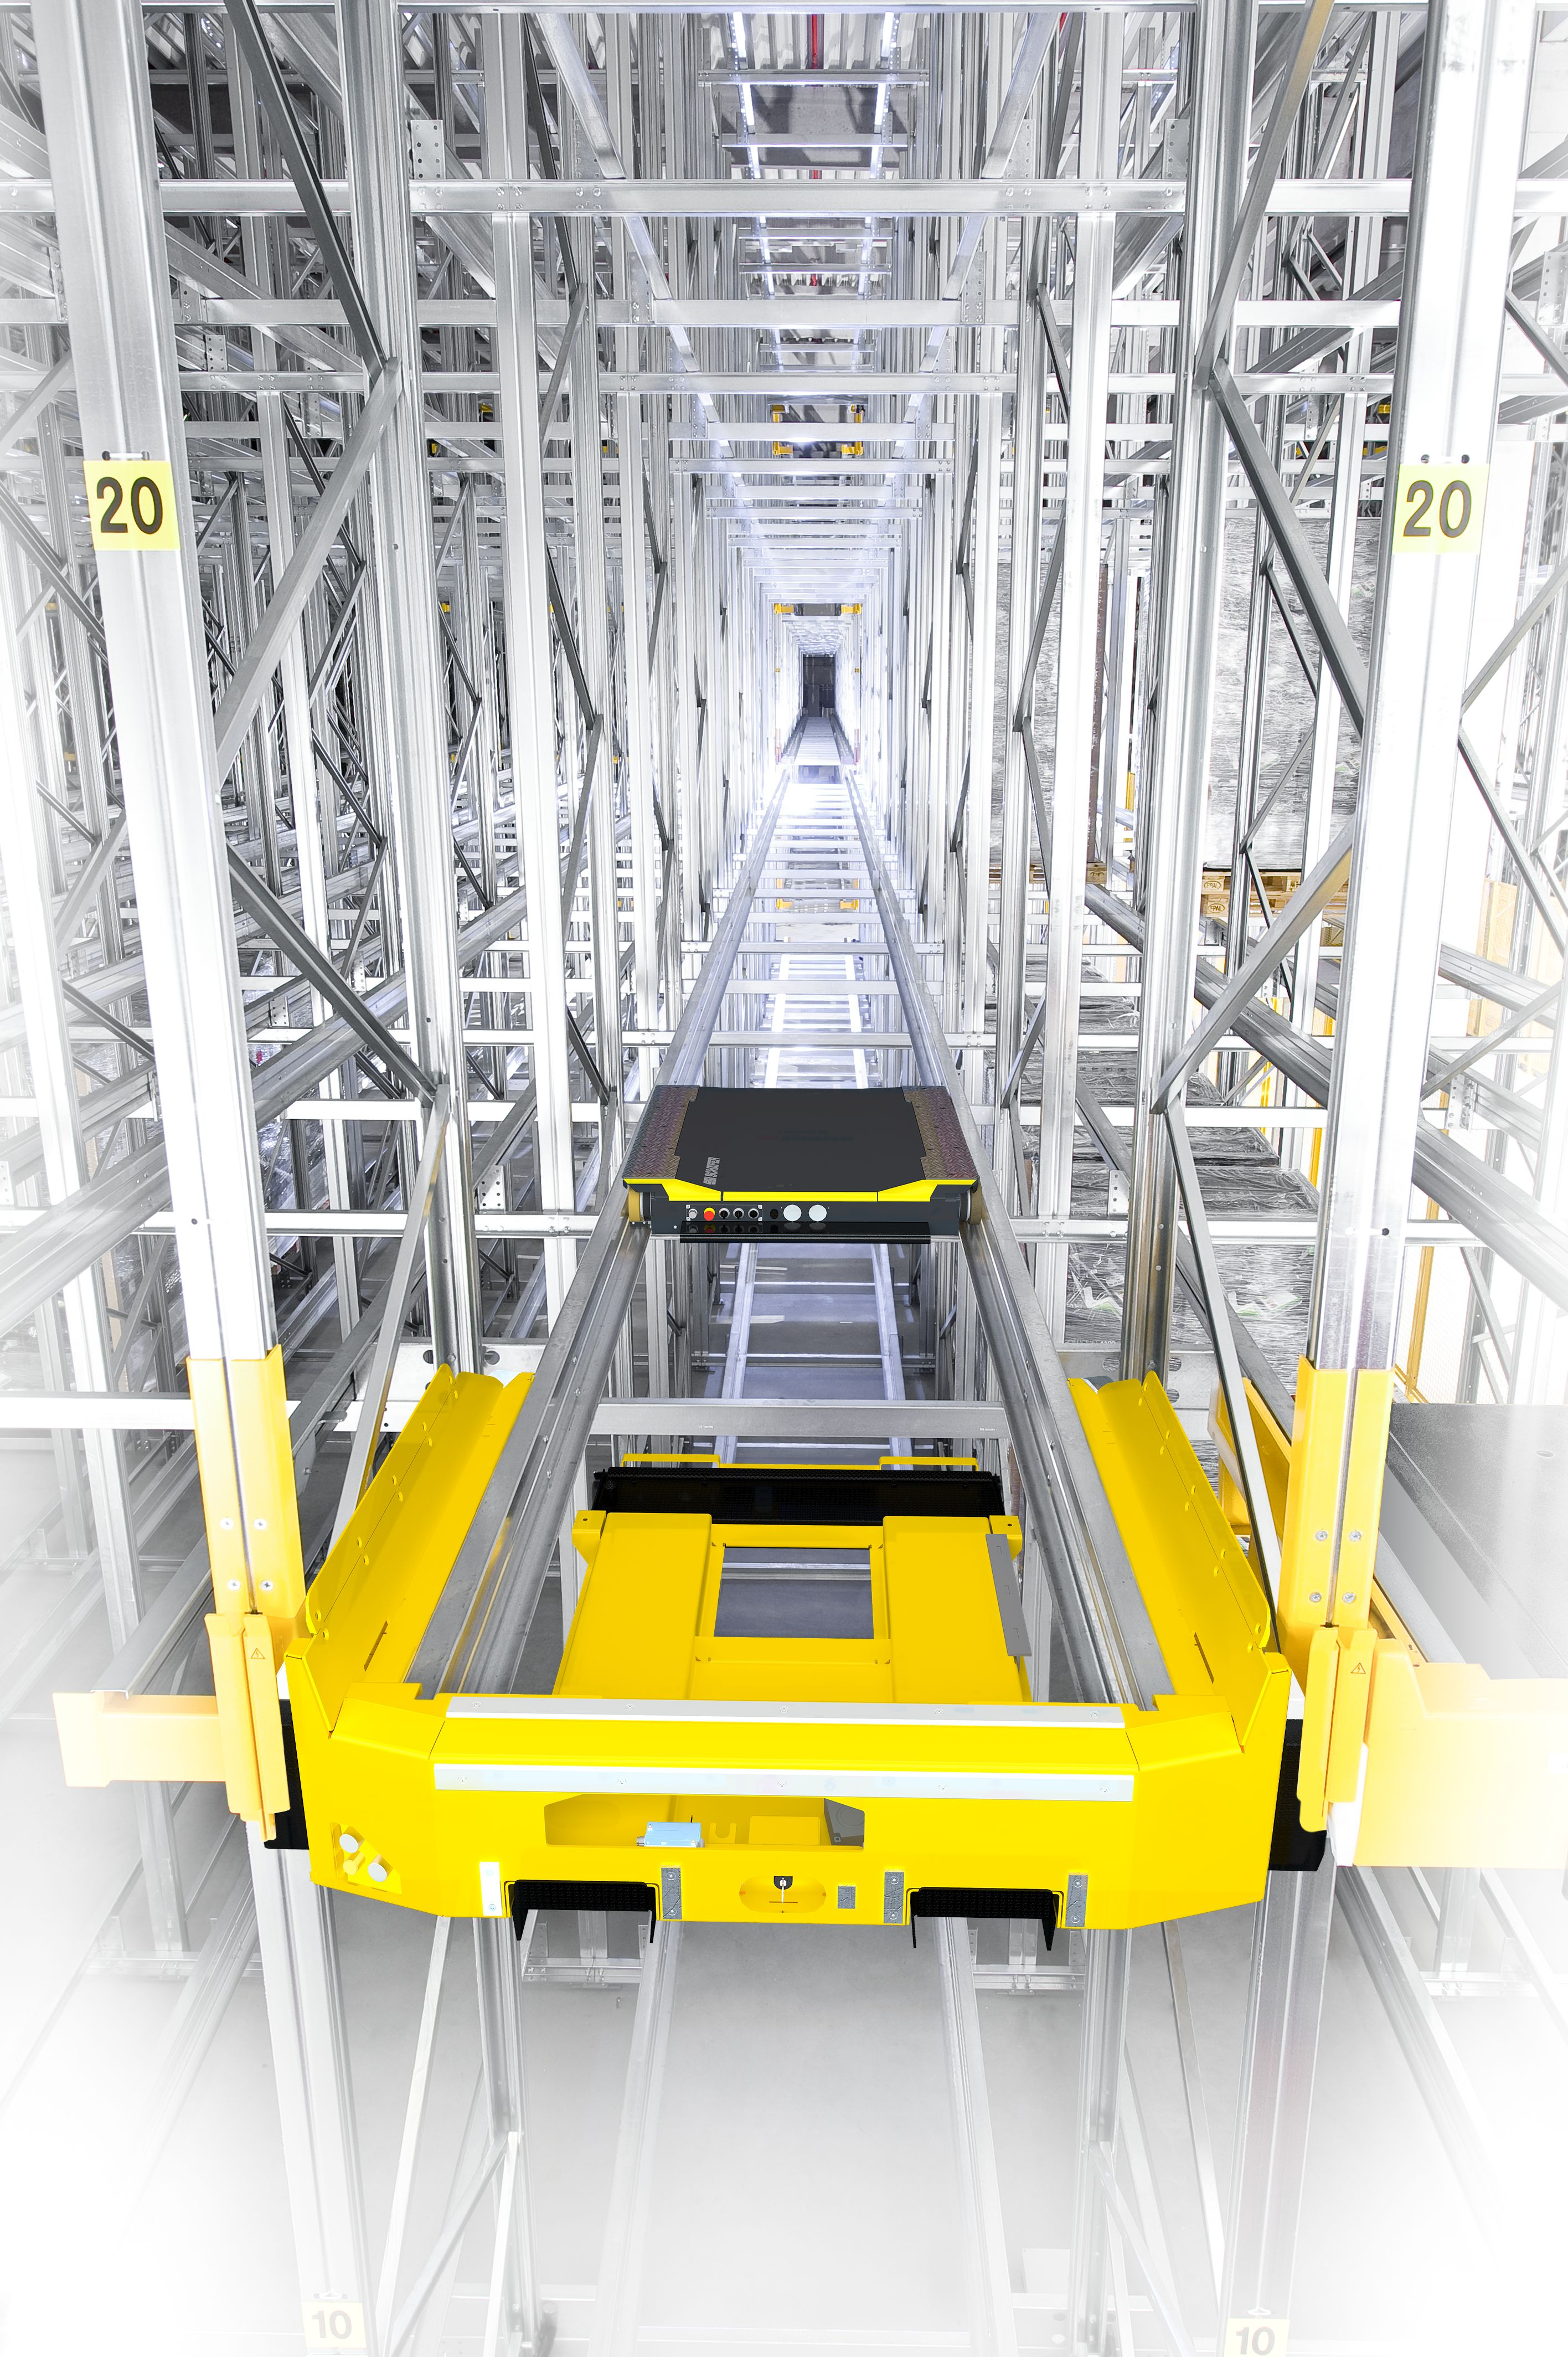
\includegraphics[width=\paperwidth,height=\paperheight]{../images/ssi_orbiter_highlight.jpg}};

			%\vspace*{1cm}

			\Huge
			\textbf{Rapport d'avancement}

			\vspace{0.5cm}
			\LARGE
			"Comment développer une application web à partir d’un client lourd déjà existant ?"

			\vspace{1.5cm}

			\textbf{Anthony PINEAU}\\
			\textbf{IR2023}

			\vfill

			
\includegraphics[width=0.6\textwidth]{../images/schaefer.jpg}
			\vfill
			
\includegraphics[width=0.4\textwidth]{../images/esaip.jpg}

			\vfill

			Période effectuée du\\
			17 avril 2023 au 19 mai 2023

			\vspace{0.8cm}
			
			\Large
			Maître de stage : Monsieur Thierry NEROT\\
			Tuteur pédagogique : Monsieur Sofiane HAMRIOUI\\
		\end{center}
	\end{titlepage}
		
	\newpage
	
	\doublespacing
	\tableofcontents
	
	\phantomsection
	\listoffigures
	\addcontentsline{toc}{section}{\listfigurename}
	
	\newpage
		
	\rfoot{Page \thepage}
	
	\singlespacing

	\section{Objectifs de la période et mise en évidence de tout changement stratégique}
		L'objectif de la période a été d'évaluer différentes solutions possibles et de choisir la plus adaptée.
		J'ai ainsi pu testé différents langages de programmation et frameworks pour développer l'application et choisir la solution qui paraît la plus adaptée pour le projet.

	\section{Travaux réalisés}
		Voici les travaux que j'ai réalise au cours de ce deuxième mois de stage :
		\begin{itemize}
			\bdot{Test du développement de l'application en delphi avec le framework TMS Software}
			\bdot{Test du développement de l'application en javascript}
			\bdot{Test du développement de l'application en ReactJS (utilisation de librairies : devextreme..)}
		\end{itemize}

	\section{Difficultés rencontrées}
		Delphi est un langage très particulier au niveau de sa syntaxe par rapport à d'autres langages plus traditionnles (java, python javascript...), de plus c'est un langage de niche où la communauté est très restreinte et il est donc parfois difficile de trouver des réponses aux problèmes rencontrés.Par ailleurs n'ayant jamais développé en react cela est parfois difficile d'appliquer correctement tous les concepts du framework qui est extrêmement complet.

	\newpage

	\section{Suite des travaux}
		\begin{figure}[h!]
			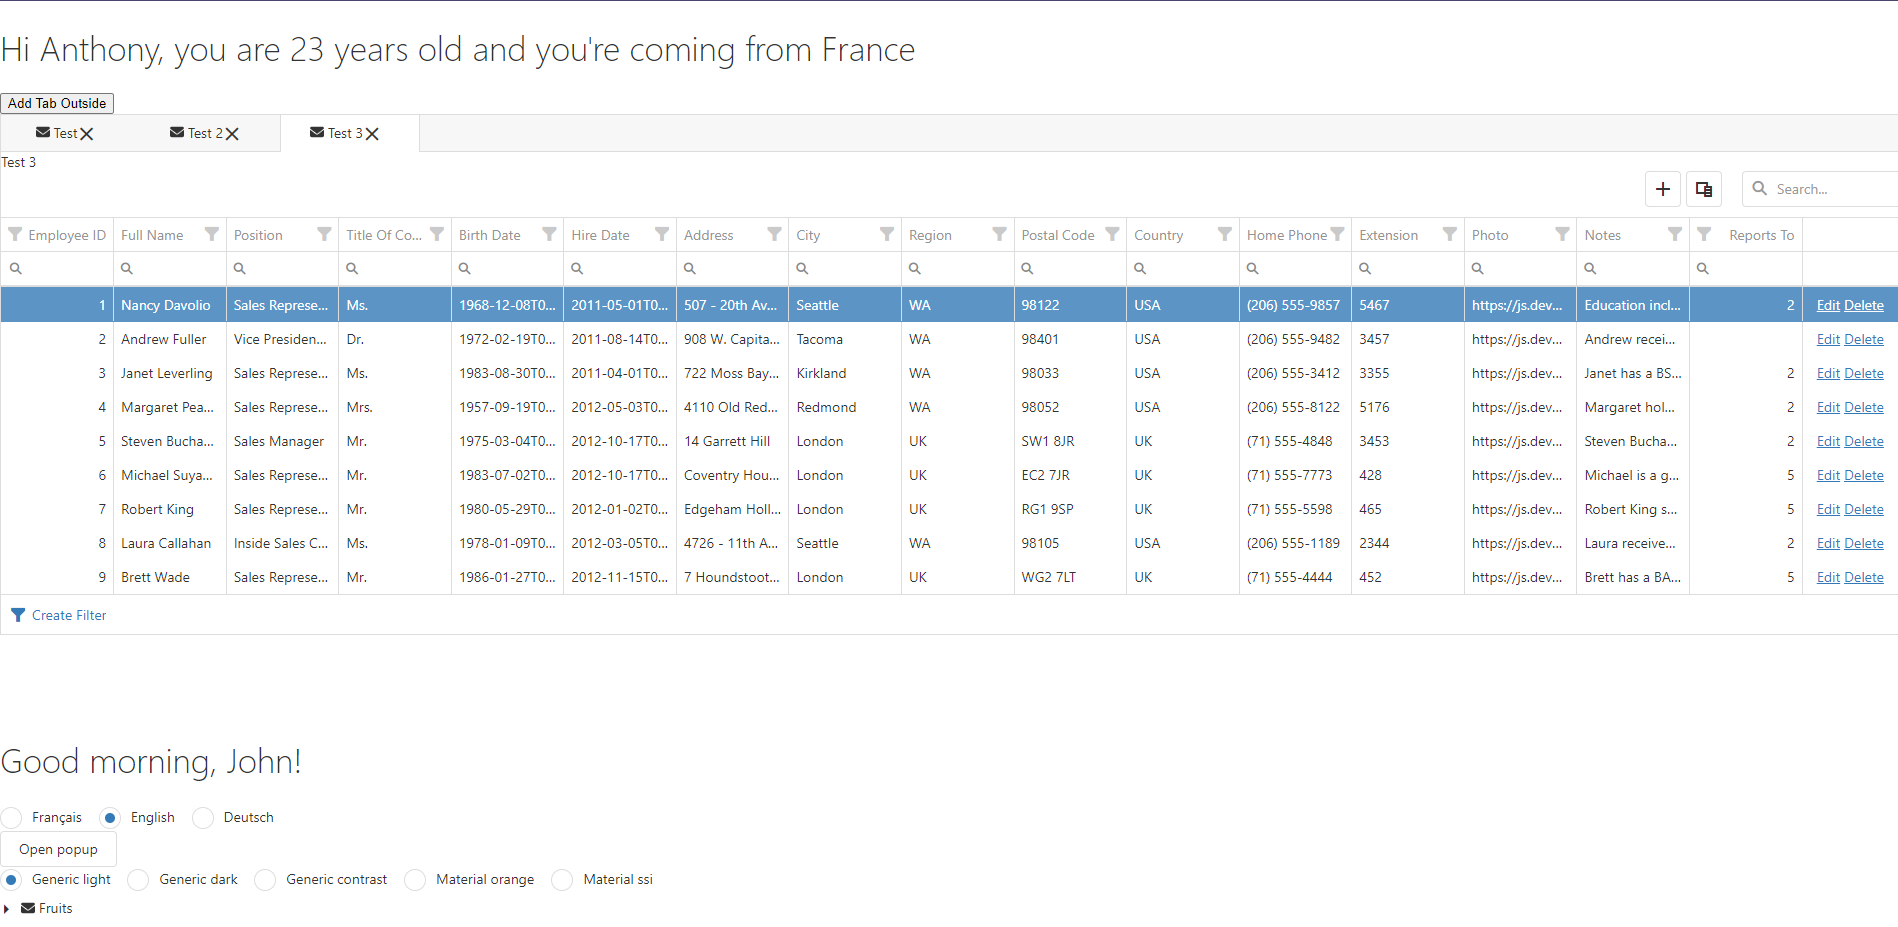
\includegraphics[width=\linewidth]{mph_web_reactts_13_04_13_05.png}
			\caption{Capture d'écran de l'application développée avec ReactJS}
		\end{figure}

	\section{Mise à jour du planning du projet}
		\begin{figure}[h!]
			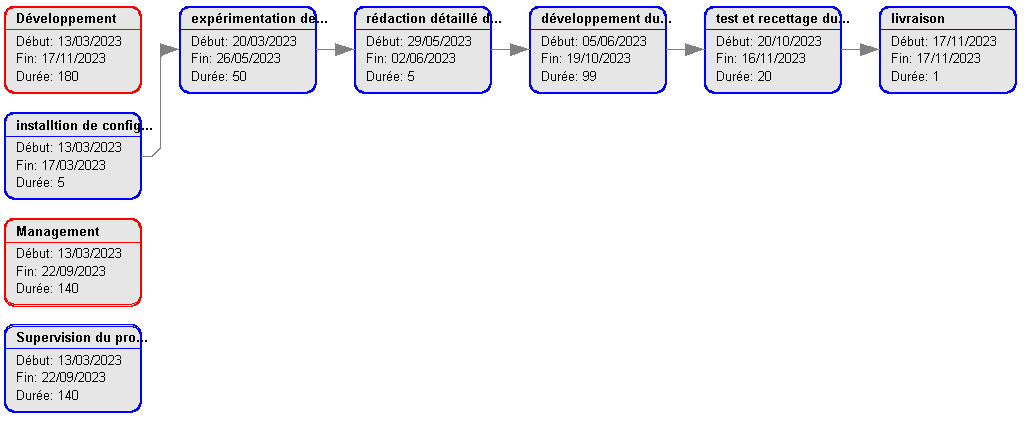
\includegraphics[width=\linewidth]{gantt_13_04_13_05.png}
			\caption{Diagramme de PERT du nouveau diagramme de GANTT pour la période du 17/04 au 19/05}
		\end{figure}
		
\end{document}